\documentclass[a4paper,12pt]{article}

\usepackage[utf8]{inputenc}
\usepackage[ngerman]{babel}
\usepackage{amsmath,amssymb}
\usepackage{graphicx}
\usepackage[a4paper, left=2cm, right=3cm, bottom=2cm]{geometry}
\usepackage{fancyhdr}
\usepackage{qrcode}
\usepackage{hyperref}
\usepackage{breakurl}
\usepackage{imakeidx}
\usepackage{wrapfig}

\graphicspath{ {./images/} }

\title{Die Atombombe}
\author{Tim, Olli, J. Z.}
\date{\today}

\begin{document}
\pagestyle{fancy}

\fancyfoot[LE,RO]{\thepage}
\fancyfoot[LO,CE]{Tim, Olli, J. Z.}
\fancyfoot[CO,RE]{Atombombe}

\maketitle

\begin{abstract}
\noindent Es wird die Entwicklung und Funktionsweise von Atombomben im 20. Jahrhundert behandelt, mit einem Fokus auf den physikalischen Prinzipien der Kernspaltung und der Erzeugung einer Kettenreaktion. Dabei werden zwei Hauptmethoden zur Erreichung der kritischen Masse vorgestellt: das Gun-Design, das in der Hiroshima-Bombe verwendet wurde, und das komplexere Implosions-Design, das bei der Nagasaki-Bombe zum Einsatz kam. Die kritische Masse ist die Mindestmenge an spaltbarem Material, die notwendig ist, um eine selbstverstärkende Kettenreaktion zu ermöglichen. Der Text erklärt auch den Unterschied zwischen unterkritischer und kritischer Masse, wobei letztere Voraussetzung für das Auslösen der Explosion ist.
\end{abstract}

\tableofcontents

\newpage

\section{Einführiung}
Die Entwicklung und der Einsatz von Atombomben im 20. Jahrhundert haben die Menschheitsgeschichte nachhaltig geprägt. Eine Atombombe basiert auf der Nutzung der enormen Energie, die bei der Kernspaltung freigesetzt wird. Im Zentrum steht die Erzeugung einer Kettenreaktion, bei der Atomkerne gespalten und dabei gewaltige Mengen an Energie in Form von Wärme, Strahlung und Druckwellen freigesetzt werden.
Zur Zündung einer Atombombe muss eine sogenannte kritische Masse erreicht werden. Dies ist die Mindestmasse an spaltbarem Material, bei der die Kettenreaktion selbstständig und unkontrolliert abläuft. Zwei Hauptmethoden zur Erreichung der kritischen Masse wurden entwickelt: das Gun-Design und das Implosions-Design.

\section{Aufbau}
\begin{wrapfigure}{r}{0.4\textwidth}
    \vspace{-1cm}
    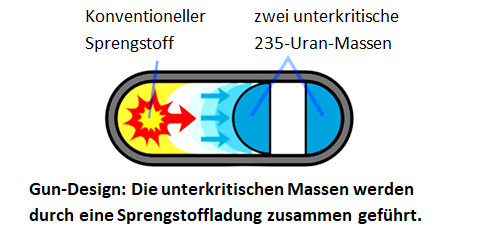
\includegraphics[scale=0.7]{Gun.png}
    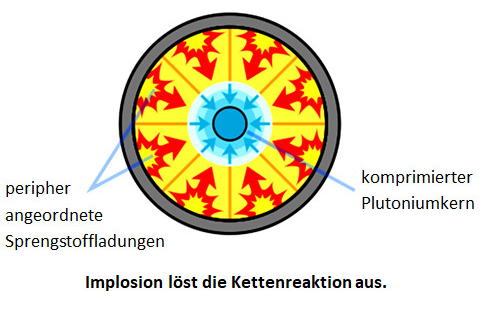
\includegraphics[scale=0.7]{Implosion.png}
\end{wrapfigure}

\textbf{Gun-Design:}
Das Gun-Design ist die einfachere der beiden Methoden und wurde bei der Hiroshima-Bombe (Little Boy) eingesetzt. Die Funktionsweise basiert darauf, 
zwei unterkritische Massen aus Uran-235 schnell zusammenzuführen (Z.b. mit TNT), um die kritische Masse zu überschreiten und die Kettenreaktion auszulösen. \hyperlink{gun_section}{Erklärung gibts auf Seite 3.}

\vspace*{2cm}

\noindent\textbf{Implosions-Design:}
Das Implosions-Design wurde bei der Nagasaki-Bombe (Fat Man) verwendet und ist deutlich komplexer als das Gun-Design. Es kommt bei Bomben zum Einsatz, die Plutonium-239 als spaltbares Material nutzen. 
Plutonium neigt bei zu langsamer Kompression zu vorzeitiger Zündung, was die Verwendung des Gun-Designs unmöglich macht. \hyperlink{implosion_section}{Erklärung gibts auf Seite 3.}

\newpage

\clearpage
\section{Funktion}
\hypertarget{implosion_section}{}
\textbf{Implosion-Design:}
Im Zentrum der Bombe befindet sich ein Plutoniumkern in unterkritischer Form.
Rings um diesen Kern sind mehrere konventionelle Sprengladungen präzise angeordnet. Diese Form ist meist kugelförmig, um eine symmetrische Druckwelle zu erzeugen.
Bei der Zündung explodieren die Sprengladungen gleichzeitig und erzeugen eine Implosion.
Der Druck komprimiert den Plutoniumkern symmetrisch nach innen, wodurch seine Dichte rapide zunimmt. Dies führt dazu, dass die kritische Masse überschritten wird.
Eine Neutronenquelle löst die Kettenreaktion aus, wodurch die Kernspaltung beginnt und Energie freigesetzt wird.

\vspace*{2cm}

\hypertarget{gun_section}{}
\noindent\textbf{Gun-Design:}
Zwei unterkritische Uran-235-Massen befinden sich an gegenüberliegenden Enden eines zylinderförmigen Bombengehäuses.
Hinter einer der Massen befindet sich konventioneller Sprengstoff (z. B. TNT).
Bei der Zündung wird der Sprengstoff detoniert und treibt eine der Uran-Massen mit hoher Geschwindigkeit gegen die andere.
Durch das Zusammenführen der Massen entsteht die kritische Masse.
Eine Neutronenquelle initiiert die Kettenreaktion, wodurch die Atomkerne gespalten und immense Mengen an Energie freigesetzt werden.

\section{Kritische-/Unterkritische Massen}
\textbf{Unterkritische Masse:}
Die unterkritische Masse ist eine Masse, bei der die Reaktion nicht nachhaltig ist. Es gibt nicht genug Material, um eine selbstverstärkende Kettenreaktion aufrechtzuerhalten. In einem unterkritischen Zustand werden weniger Neutronen freigesetzt, als benötigt werden, um eine fortgesetzte Kettenreaktion zu ermöglichen.

\vspace*{2cm}

\noindent\textbf{Kritische Masse:}
Die kritische Masse bezeichnet die Mindestmenge an Material, die erforderlich ist, damit eine nukleare Kettenreaktion selbstständig ablaufen kann. Für spaltbares Material wie Uran oder Plutonium bedeutet dies, dass die Anzahl der Neutronen, die bei jeder Spaltung freigesetzt werden, ausreicht, um weitere Spaltungen zu verursachen und so eine unaufhörliche Reaktion zu ermöglichen.
Die kritische Masse lässt sich wie folgt bestimmen:

\begin{equation}
    \fontsize{20}{10}
    M_\text{krit} = \frac{4}{3} \pi R^3 \rho
    \label{eq:kritische_masse}
\end{equation}

\newpage
\clearpage

\section{Tabelle: Materialeigenschaften}
\begin{table}[h]
    \centering
    \begin{tabular}{|c|c|c|}
    \hline
    Material & Kritische Masse (kg) & Spaltbares Isotop \\
    \hline
    Uran-235 & 52 & Ja \\
    Plutonium-239 & 10 & Ja \\
    Thorium-232 & 230 & Nein \\
    \hline
    \end{tabular}
    \caption{Eigenschaften verschiedener Materialien}
\end{table}

\newpage

\section{Links}
\begin{center}
    \qrcode{https://github.com/Jason4225/LaTeX-Atombombe}
\end{center}
\bigskip

\href{https://github.com/Tim-foe}{Github: Tim} \hspace{4cm}
\href{https://github.com/YoOlli}{Github: Olli} \hspace{4cm}
\href{https://github.com/Jason4225}{Github: J. Z.}

%\bibliographystyle{plain}
%\bibliography{bibliography.bib}

\end{document}